\chapter{MODELING WITH CONNECTED MATCHINGS}


\section{Bipartite graphs}
	In a typical bipartite matching problem, we are attempting to perform an {\it assignment}.  We are given a collection $A$ of one type of object, a collection $B$ of a second type of object, and a set of feasible assignments
of objects from $B$ to each object in $A$.  We assume that only one object may be assigned to another object.  The problem is to choose from among these possible assignments a set of {\it actual} assignments that maximizes some desirable property.
	
	In the case of {\it connected} matchings, we have added another requirement.  The assignment must be done in such a way that among the objects in any two assigned pairs, there is some other, unused feasible assignment.  This may model redundancy, flexibility, interconnectivity, proximity, or some other quality we wish to demand of the chosen matching.   
	\subsection{Cloud administration}

	Let us draw up a hypothetical problem that highlights the above description.  Suppose we are administering a cloud-based application. Broadly speaking, the architecture of the application consists of {\it servers} which store and process data and {\it clients} which deliver content and receive commands from end users.  At any given time, each client is logged in to the small subset of servers needed to carry out a particular task.

Suppose that we want to allow limited and moderated client-client communication.  For privacy, security, or other reasons we do not wish to allow all clients logged in to a given server to send and receive messages from each other.  In fact, we require that one side of any transmission be a superuser.   This privileged client serves to moderate the communication.  However, we do wish for {\it any} two clients logged into {\it any} of the servers to be able to get a message from one to the other as quickly as possible. 

We begin with a matching problem: how do we assign a privileged (logged-in) client to each server?  Each superuser will administer its assigned server, in addition to transmitting messages among clients logged into that server.  By itself, this question provides us with a collection of superusers that can moderate all messages on any given server.  Furthermore, each message passes through only one intermediary.  This is close to what we want, but so far we cannot guarantee that users not mutually logged into any particular server can communicate.

To fully meet our requirements, we must ensure that there is a ``safe'' path between any two servers.  To meet them and ensure rapid communication, we should ensure that any pair of superusers are both logged into some server and can thus pass messages.  When we make an assignment that does so, we have actually found a {\it connected} matching.  It is also not difficult to see that any connected matching in the server-client bigraph represents a satisfactory assignment of servers to superusers. 

An interesting feature of this particular example is an asymmetry in scaling.  As the application grows in users, each individual server machine will be able to serve greater numbers of clients, provided that the software involved is well designed and scalable.  If the number of servers remains essentially fixed as the application grows, then we will still be able to efficiently identify large connected matchings in the server graph.
	\subsection{The bipartite margin shop}

Another application of connected matchings in bipartite graphs arises from the work of Oron, Steiner and Timkovsky in \cite{OST}.  A large brokerage firm may manage tens of millions of customer accounts.  Margining these accounts and producing account status slips at the end of each business day presents a serious computational challenge.  Oron et. al model the computational task with a graph they term the {\it bipartite margin shop}.

A bipartite margin shop $G = (A, B; E)$ is a bipartite graph with vertices that represent tasks.  Each task $v$ has an associated processing time $p_v$.  Each connected component of this graph is called a {\it job}.  This graph is a {\it precedence graph} \index{Precedence graph} in that an edge $ab$, with $a \in A$ and $b\in B$, is present when task $a$ must be completed no later than task $b$.  This model is bipartite on the assumption that there are two machines at work, $M_A$ and $M_B$.  Tasks from $A$ are processed on machine $M_A$, and tasks from $B$ are processed on machine $M_B$.  Interpreting this problem in terms of a brokerage firm margining accounts,we have an edge between the tasks $a$ and $b$ if the account $b$ has a position in the security $a$. This means the ``market'' machine $M_A$ must calculate the margin requirement for one unit of the security $a$
before the ``account'' machine $M_B$ can calculate the margin requirement for the account $b$.

In the margin-shop scheduling problem, we take a bipartite margin shop and try compute to the schedule that completes each job in the minimum time without violating the precedence relationships encoded in the graph.  The authors of \cite{OST} prove that the bipartite margin shop problem is actually equivalent to the MR problem discussed in Chapter 4.


\begin{figure}
	\begin{center}
	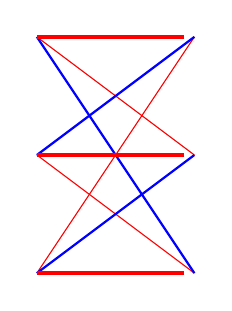
\begin{tikzpicture}[thick,scale=1]

\draw[color = red, thin] (-1,2.5)--(1,1);
\draw[color = red, thin] (-1,1)--(1,-.5);
\draw[color = red, thin] (-1,-0.5)--(1,2.5);
\draw[color = blue] (-1,2.5)--(1,-0.5);
\draw[color = blue] (-1,1)--(1,2.5);
\draw[color = blue] (-1,-0.5)--(1,1);

\draw (1, 2.5) node[]{}
	edge[color = red, ultra thick] (-1, 2.5);
\draw (-1, 2.5) node[]{};
\draw (1, 1) node[]{}
	edge[color = red, ultra thick] (-1, 1);
\draw (-1, 1) node[]{};
\draw (1, -0.5) node[]{}
	edge[color = red, ultra thick] (-1, -0.5);
\draw (-1, -0.5) node[]{};


\end{tikzpicture}
	\end{center}
	\caption{A red connected matching $M$ with an alternating cycle of length six.}
	\label{rb_cexp}
\end{figure}
This is very closely related to the problem of finding a connected matching in the graph of red edges.  In fact, a matching as described above with no alternating blue-red cycles would certainly be a connected matching.  As we proved in Chapter 4, for chordal bipartite graphs, the problems are equivalent.  However for general bipartite graphs it is stronger than the notion of a connected matching.  As we see in Figure \ref{rb_cexp}, a connected matching in red edges could permit alternating cycles longer than four edges.  

\section{General graphs}

Sometimes we may encounter a matching-type problem with only one type of object modeled by nodes.  In this case, we cannot assume that the appropriate graph model is bipartite.  The relation we wish to model with edges in the graph is assumed to be non-transitive, as otherwise the graph model degenerates into a collection of disconnected cliques.
	\subsection{Partnership assignments}
One type of ``assignment between equals'' we encounter in the real world is that of working partnerships.  In any organization, we can model individuals as vertices in a graph and use edges to represent some type of advantageous (non-transitive) working relationship.  By identifying a connected matching, we collect a set of possible partnerships wherein each pair of partners has the advantageous relationship and any two pairs $A$ and $B$ have an indvidual from pair $A$ that has the advantageous relationship with some individual from pair $B$,

Let us see how this might work in a high school mathematics classroom.  Suppose we model the students in the class as vertices. We are interested in the opportunities students have to work together outside of class, so we place an edge between vertices if the corresponding students share a study hall, lunch period, or live within a block of one another.  We want to assign a project to groups of two students each, and would like for the students to have time to work on the project outside of class.  Assigning groups so that each group corresponds to an edge in the graph we have constructed is a matching problem, and the result is a collection of pairs of students that have opportunities to work together outside of class.  

Now let's suppose that the content of each pair's assigned project is a piece of a larger class project.  In light of this, we would like to additionally require that each pair of two-student groups has a chance to share their findings and collaborate outside of class.  In order for this to happen, the matching must also be connected.  That is to say, in any two groups $A$ and $B$, there is a student from $A$ who shares a study hall, lunch period, or neighborhood with a student from $B$.  


	